\section{Sc}
В данном разделе представлены основные понятия из Sc, которые требуются для понимания предметной области с которой работает JMantic. 

\subsection{Введение}

В библиотеке JMantic есть 1 супертип - sc-элемент, и 3 конкретных типа sc-элемента. 

\subsubsection{ScElement}
Любой объект в sc-памяти является ScElement. Характеризуется данный тип наличием sc-адреса, то есть, адреса сущности в sc-памяти. Sc-адреса в рамках одной базы уникальны.

\subsubsection{ScNode}
Данная сущность расширяет ScElement добавлением типа. ScNode может иметь тип константности, переменности и т.д. Однако, JMantic любую ScNode обрабатывает единым образом, вне зависимости от её типа. 

\subsubsection{ScEdge}
ScEdge также, как и ScNode имеет тип. Однако, кроме типа, ScEdge соединяет две любые сущности ScElement.

\subsubsection{ScLink}
ScLink предназначена для хранения информации в sc-памяти. На данный момент доступно 4 формата сохранения информации: Целые числа, Дробные числа, Строки, Бинарная информация (не реализовано в JMantic). 
Для каждого типа информации (кроме бинарного) в библиотеке JMantic есть соответствующий интерфейс. 

\subsection{Описание структуры языка SC}

Язык SC(Semantic Code) - это расширение языка SCB(Semantic Code Basic) путем включения в число текстовых элементов не только знаков множеств, но и переменных. Таким образом, элементы, входящие в состав sc-текстов (т.е. sc-элементы) делятся на следующие классы:

\begin{itemize}
\item sc-константы (константные sc-элементы; sc-элементы, являющиеся знаками множеств; sc-элементы, каждый из которых имеет одно значение, каковым является сам этот элемент; sc-элементы нулевого уровня; scb-элементы); 
\item просты sc-переменные (sc-элементы, значениями которых являются sc-константы; sc-элементы 1-го уровня; sc-переменные 1-го уровня);
\item sc-метапеременные (sc-элементы, значениями которых являются sc-переменные; sc-элементы 2-го уровня).
\end{itemize}

В свою очередь, sc-переменные разбиваются на следующие подклассы:

\begin{itemize}
\item переменные, значениями которых являются знаки множеств неуточняемого типа;
\item переменные, значениями которых являются знаки пар принадлежности;
\item переменные, значениями которых являются знаки узловых множеств;
\item метапеременные, значениями которых являются переменные, значениями которых являются знаки множеств неуточняемого типа;
\item метапеременные, значениями кторых являются перменные, значениями которых яляются знаки пар принадлежности;
\item метапеременные, значениями которых являются перменные, значениями которых являются знаки узловых множеств.
\end{itemize}

Язык SC, как и язык SCB, имеет две модификации - язык SCs (Semantic Code string) и язык SCg (Semantic Code graphical).

Вводятся также ребра, указывающие на совпадение либо возможные совпадения значения некоторой переменной со значениями переменной или константы.

\subsection{Язык SCg (Semantic Code Graphical) - графическая модификация языка SC}

Так как набор элементов языка SC по сравнению с языком SCB значительным образом расширен, то
его графическая (нелинейная) модификация требует введения дополнительных графических
примитивов для изображения различных типов sc-элементов. В связи с этим в языке SC приняты
следующие соглашения: 
\begin{itemize}
    \item константные sc-элементы неуточняемого типа и константные sc-узлы изображаются кружочками;
    \item переменные sc-элементы неуточняемого типа и переменные sc-узлы изображаются квадратами, ориентированными по вертикали и горизонтали;
    \item изображение sc-метапеременных отличается тем, что изображающий их квадрат повернут на 45 градусов;
    \item изображение sc-элементов неуточняемого типа от изображения sc-узлов отличается уменьшенным размером;
    \item изображения дуг и ребер, являющихся константами, простыми переменными и метапеременными, отличаются друг от друга тем, что константные дуги и ребра представлены сплошными линиями (того или иного вида), простые перменные - пунктирными линиями, а метапеременные - штрих-пунктирными линиями.
\end{itemize}

\subsection{Основные графические примитивы языка SC}
 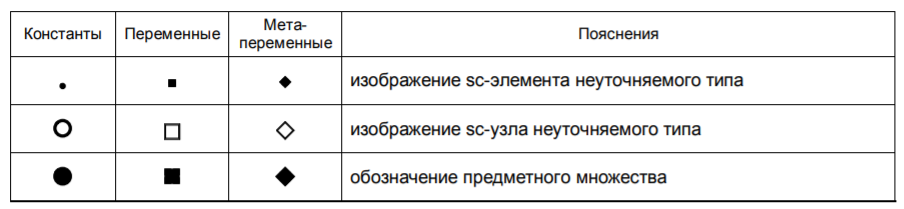
\includegraphics[scale=0.5]{images/sc1.png}
 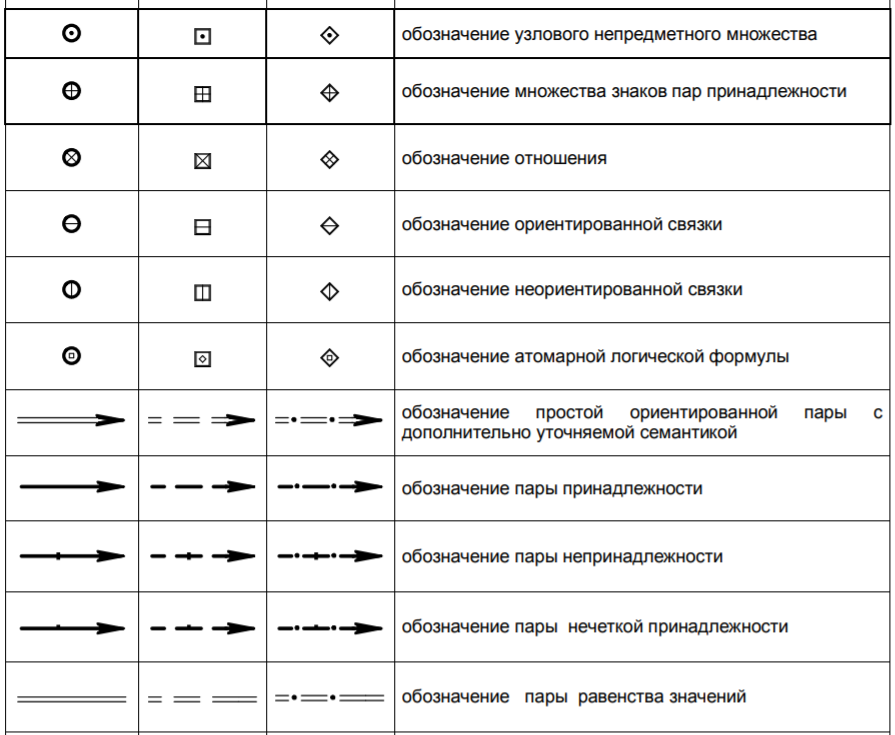
\includegraphics[scale=0.5]{images/sc2.png}
 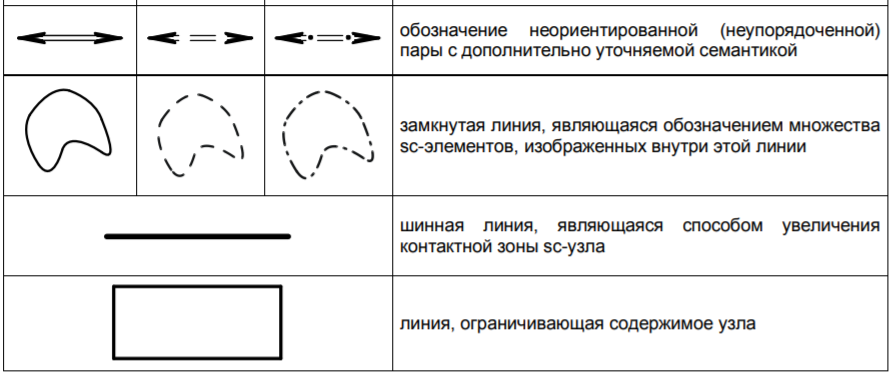
\includegraphics[scale=0.5]{images/sc3.png}
 
 \subsection{Язык SCs (Semantic Code string) – линейная модификация языка
SC}

 В число разделителей и ограничителей языка SCs входят все разделители и ограничители языка SCBs. Кроме этого, к указанному перечню разделителей и ограничителей добавляются новые:
 
 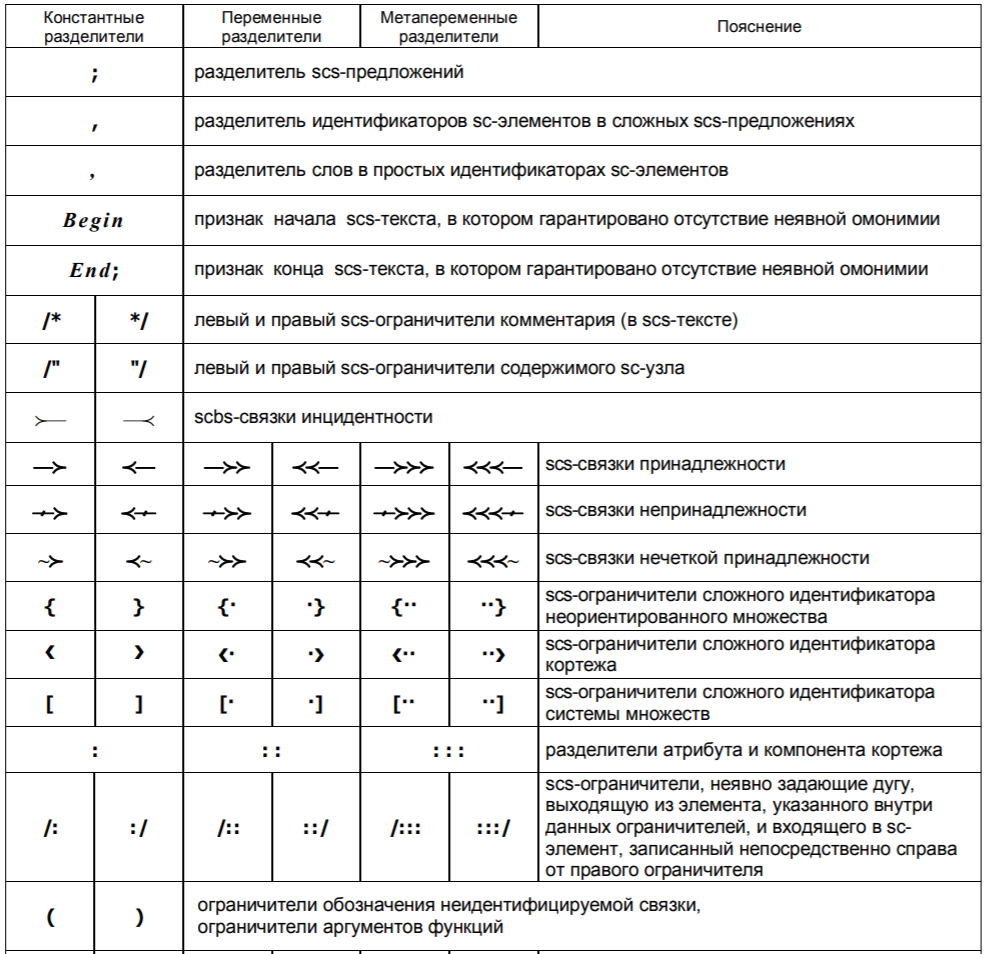
\includegraphics[scale=0.48]{images/sc4.png}
 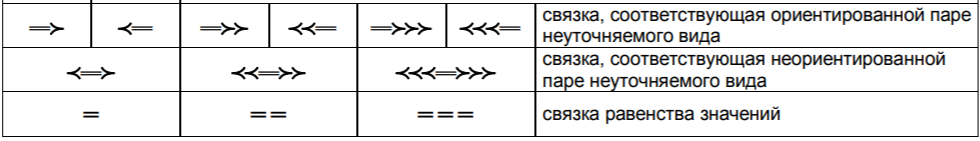
\includegraphics[scale=0.48]{images/sc5.png}
 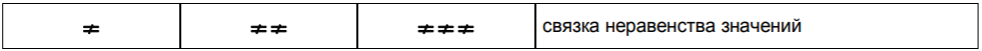
\includegraphics[scale=0.48]{images/sc6.png}
 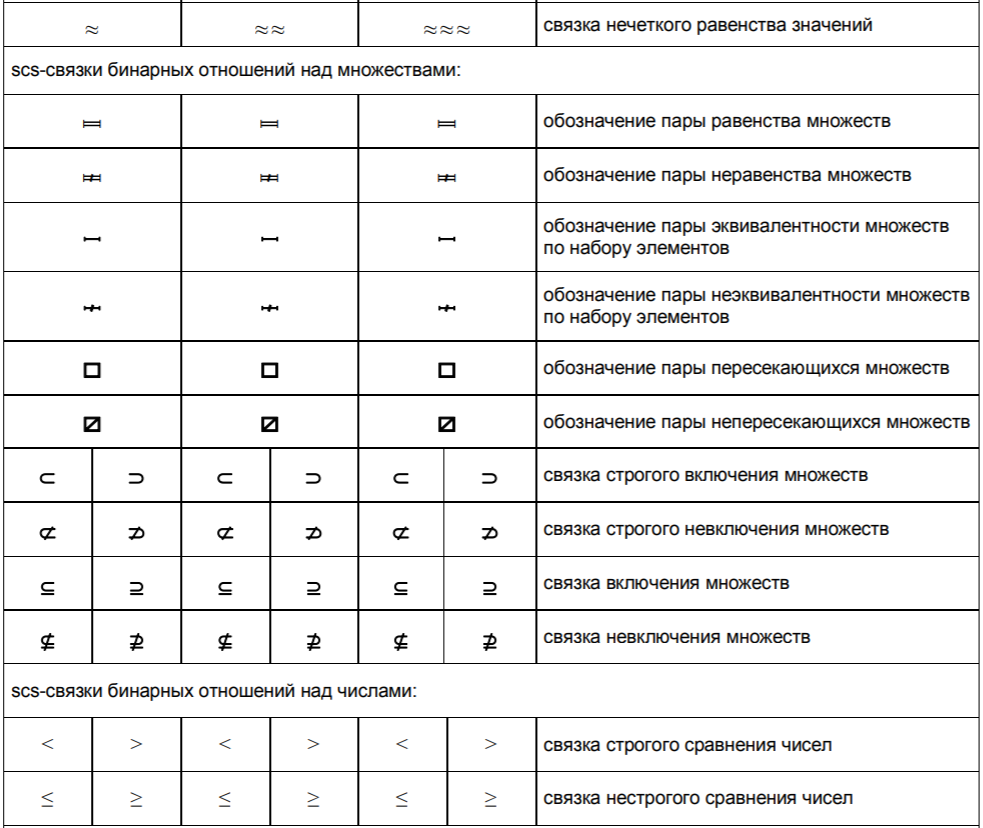
\includegraphics[scale=0.48]{images/sc7.png}
 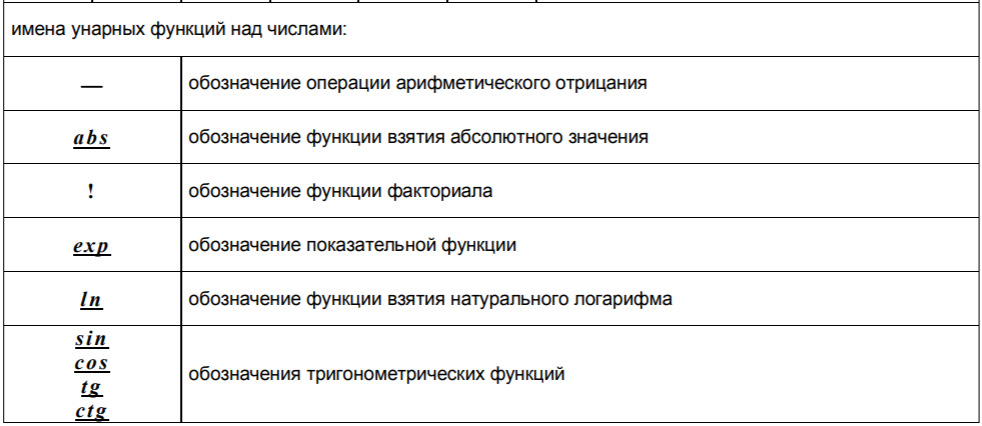
\includegraphics[scale=0.48]{images/sc8.png}
 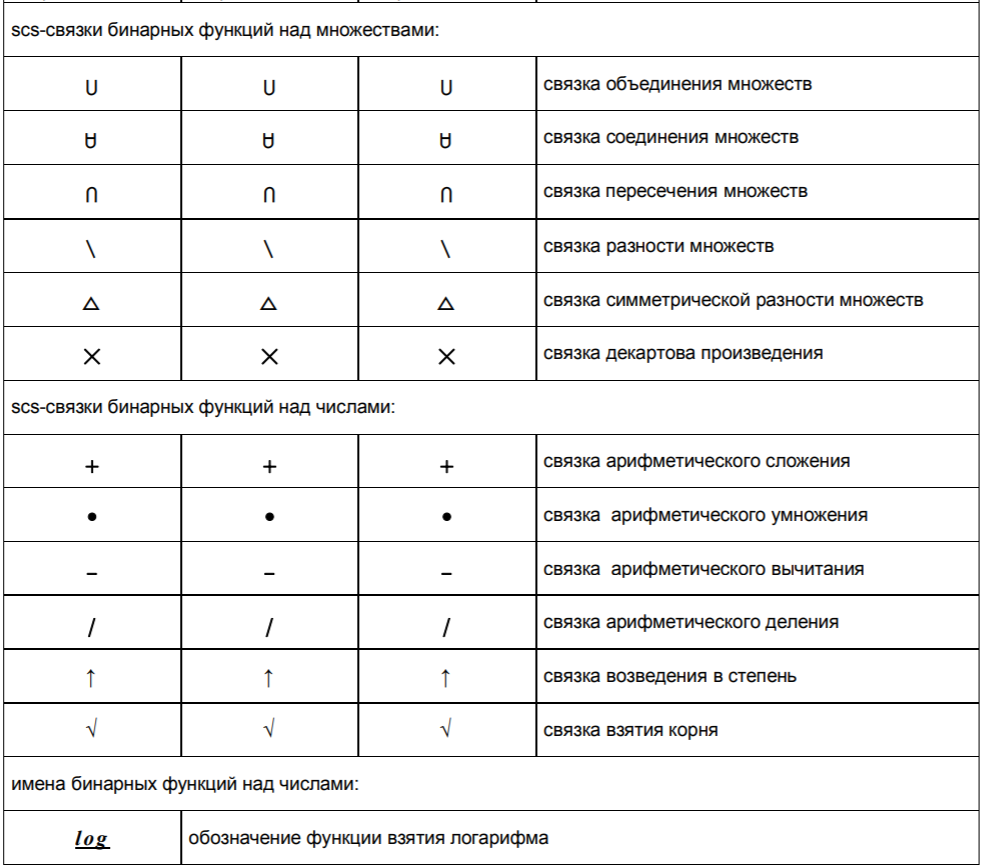
\includegraphics[scale=0.48]{images/sc9.png}
 
 \subsection{Простые примеры для понимания сущности SC языка}
 \subsubsection{Пример на языке SCs:}
 
 В данном примере можно наглядно увидеть, как можно описать понятие "Устройство на языке SCs, конечно, не в полной мере, но в общих чертах однозначно.
 
Конкретно здесь мы видим, что устройство включается в такое понятие, как изобретение. А также есть ссылка на файл, в котором находится определение этого понятия на русском языке: рукотворный объект со сложной внутренней структурой, 
созданный для выполнения определённых функций.
  
 \begin{lstlisting}[language=json,firstnumber=1]
concept_device

    <= nrel_inclusion: concept_invention ;

    => nrel_main_idtf:
        [Device]
        (*<-lang_ru;;*);
        [Device]
        (*<-lang_en;;*);

    => nrel_idtf:
        [device]
        (*<- lang_ru;;*);

    <- rrel_key_sc_element: ...
        (*
            <- definition;;

            => nrel_main_idtf:
                [Definition.(Device)]
                (*<-lang_ru;;*);;

            <= nrel_sc_text_translation: ...
                (* 
                    -> rrel_example: 
                        "file://html/concept-device.html"
                        (*<-lang_ru;;*);; 
                *);;

            <= nrel_using_constants: ...
                (*
                    -> subject;; //ims
                    -> _structure;; //ims
                    -> concept_function;;
                *);;
        *);;
\end{lstlisting}
Содержимое файла, соответствующее пути в примере:

Устройство --— это рукотворный объект со сложной внутренней структурой, 
созданный для выполнения определённых функций.</p>

\newpage

\subsubsection{Пример на языке SCg}

Для пример на SCg было взято такое музыкальное направление как "Регги", на рисунке мы можем видеть, что Регги - это музыкальное направление, которое зародилось в такой стране, как Ямайка. Также здесь показано, что Боб Марли, певец и автор песен, является королём этого жанра.

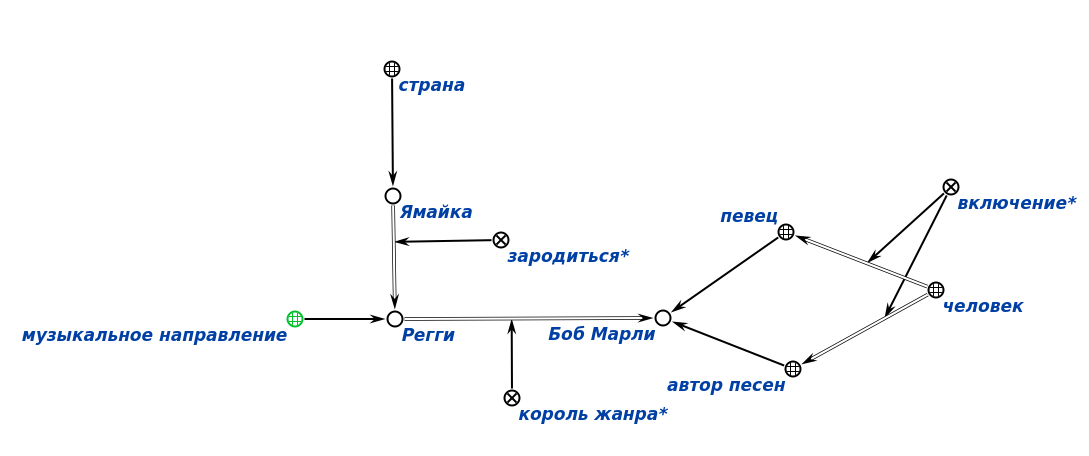
\includegraphics[scale=0.4]{images/sc10.png}

 Также на языке SCg можно описывать и математические выражения.
 В примере описано выражение (a+b) в степени 3:
 
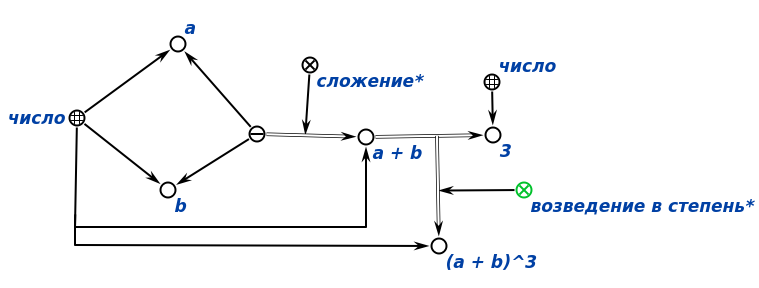
\includegraphics[scale=0.5]{images/sc11.png}


